\chapter{Implementation}
\label{ch:impl}

\section{Implementation and Engineering}
This chapter describes how the design of Chapter~\ref{ch:design} was realised: the environment, the module structure, the algorithms, the training
and evaluation tooling, the dashboard, the tests and the deployment. All code is in the project repository; key excerpts are listed in
Appendix~\ref{app:code}.

\subsection{Development Environment Setup}
The backend is a Python package (\code{backend/verifai}) installed from \code{requirements.txt}; training and development extras are
separate files. Configuration is read from environment variables or an optional \code{.env} file so that the same code runs locally, in
Docker and on a hosting service. The frontend (\code{frontend/}) is built with Vite and served either by the API process (single-container
mode) or by a static host. Typical commands are:

\begin{lstlisting}[language=bash,numbers=none,caption={Running the project locally.},label={lst:run}]
cd backend && python -m venv .venv && .venv\Scripts\activate
pip install -r requirements.txt
cd ../frontend && npm ci && npm run build
cd ../backend && set VERIFAI_FRONTEND_DIR=..\frontend\dist
python -m uvicorn verifai.api.app:app --host 127.0.0.1 --port 8000
\end{lstlisting}

\begin{table}[ht]
\centering
\caption{Core modules and file structure of the repository.}
\label{tab:modules}
\small
\begin{adjustbox}{max width=\linewidth,center}
\begin{tabular}{|p{4.4cm}|p{7.4cm}|}
\hline
\textbf{Module / path} & \textbf{Responsibility} \\ \hline
\code{verifai/config.py} & Settings from environment variables; default model order; limits \\ \hline
\code{verifai/model.py} & \texttt{SRMLayer}, \texttt{TwoStreamNet}, safe checkpoint loading, thread-safe prediction \\ \hline
\code{verifai/preprocess.py} & JPEG round-trip and ImageNet normalisation shared by training and inference \\ \hline
\code{verifai/faces.py} & MTCNN detection with confidence and size filters; box overlap for tracking \\ \hline
\code{verifai/registry.py} & Model registry: default / alternative / rollback roles, per-analysis selection, model identification \\ \hline
\code{verifai/scoring.py} & Labels, INCONCLUSIVE band, decisiveness, aggregation, temporal statistics, suspicious segments \\ \hline
\code{verifai/image_pipeline.py}, \code{video_pipeline.py} & Image and video analysis; evidence artifacts \\ \hline
\code{verifai/explain.py} & Grad-CAM on the RGB stream's last block \\ \hline
\code{verifai/report.py} & PDF forensic report \\ \hline
\code{verifai/store.py}, \code{engine.py} & Result storage, retention, background jobs, cancellation \\ \hline
\code{verifai/api/app.py} & FastAPI application, upload validation, routes, CORS \\ \hline
\code{training/} & Data preparation and validation, training, evaluation, degradations, stream ablation, quality bins, acceptance gate, modern-generator data \\ \hline
\code{frontend/src/} & Pages, result viewers, upload card, history, API client, tests \\ \hline
\code{kaggle/} & Builders for the private GPU notebooks \\ \hline
\code{docs/} & Architecture, evaluation, dataset, API, guides and experiment records \\ \hline
\end{tabular}
\end{adjustbox}
\end{table}

\subsection{Algorithm Specifications}
The operational logic is governed by three procedures. They make explicit the order of preprocessing and the way scores are aggregated.

\begin{algorithm}[ht]
\caption{Image analysis}
\label{alg:image}
\begin{algorithmic}[1]
\Require image file $I$, settings $S$, model $M$
\Ensure label and score for $I$, per-face results, evidence images
\State $rgb \gets \textsc{DecodeAndValidate}(I)$ \Comment{format, size, pixel limits}
\State $faces \gets \textsc{DetectFaces}(rgb)$ \Comment{MTCNN; keep conf $\ge0.90$, side $\ge32$\,px; at most 10}
\If{$faces=\emptyset$} \State \Return INCONCLUSIVE \Comment{no usable face is a result, not an error} \EndIf
\State $X \gets \textsc{Normalise}(\textsc{JpegRoundTrip}_{q=95}(\textsc{Crop}_{224}(faces)))$
\State $p \gets M(X)$ \Comment{raw sigmoid score per face}
\State $maps \gets \textsc{GradCAM}(M.\text{rgb\_stream},X)$ \Comment{skipped if unavailable}
\State $p_{img} \gets \max_i p_i$; \; $label \gets \textsc{Classify}(p_{img},\text{margin}=0.15)$
\State store annotated image, face crops, heat-maps; \Return $(label,p_{img})$
\end{algorithmic}
\end{algorithm}

\begin{algorithm}[ht]
\caption{Video analysis (background job)}
\label{alg:video}
\begin{algorithmic}[1]
\Require video file $V$, sampling rate $\approx2$\,fps, frame cap $64$
\Ensure verdict, tracks, suspicious ranges, evidence frames
\State $frames \gets \textsc{SampleFrames}(V)$; skip corrupt frames
\For{each frame $f$}
  \State $faces_f \gets \textsc{DetectFaces}(f)$; assign each face to a track by box overlap
\EndFor
\State score all face crops in batches; $s_f \gets \max$ face score in frame $f$
\State for every track with $\ge3$ observations: $s_{track} \gets \operatorname{median}$ of its scores
\State $p_{video} \gets \max_{track} s_{track}$ \Comment{pooled fallback when no track is long enough}
\State $ranges \gets$ maximal runs of consecutive frames with $s_f>0.5$
\State $E \gets$ six frames with highest $s_f$; store frame with boxes and Grad-CAM of its top face
\State \Return $(\textsc{Classify}(p_{video}),\ tracks,\ ranges,\ E)$
\end{algorithmic}
\end{algorithm}

\begin{algorithm}[ht]
\caption{Selecting what the frame viewer shows}
\label{alg:viewer}
\begin{algorithmic}[1]
\Require selected frame index $i$, analysed frames $F$, stored evidence $E$ (frame image, optional heat-map)
\State $e \gets E[i]$ if present
\If{$e$ exists}
  \State show the stored frame (with face boxes); show $e$.heatmap if it exists, else say ``not generated''
\Else
  \State say ``no frame image or heat-map was stored for this timestamp''; offer the nearest stored frame \Comment{nothing is approximated}
\EndIf
\State selecting a timestamp range $r$: choose the stored evidence frame with the highest score inside $r$, else the highest-scoring analysed frame
\end{algorithmic}
\end{algorithm}

\subsection{Module-wise Implementation Breakdown}
\textbf{Face localisation and normalisation.} Detection uses the pre-trained MTCNN of \citep{zhang2016mtcnn} through the
\texttt{facenet-pytorch} package. Detection runs on a downscaled copy for speed; boxes are scaled back and crops are cut from the original
image. The same detector produced all training crops.

\textbf{Model loading.} Checkpoints are loaded with weights-only deserialisation and strict key matching, so a mismatching file raises an error instead
of silently loading partial weights. Both the original prototype's raw state dictionaries and the new files with metadata are accepted. The
SHA-256 of the checkpoint is computed at load time and recorded in every result.

\textbf{Model registry.} The registry knows E4, Model 4 and v2. The server loads one default model at start-up (E4 locally; the hosted image pins v2); another model is loaded on first use and at most one such model stays in memory. \code{GET /api/models} lists the models with their roles, the analysis endpoints accept a \code{model} field, and every result, dashboard chip and PDF report records the model name, role, status note and checkpoint hash.

\textbf{Scoring and aggregation.} Labels use the fixed 0.5 threshold and the $\pm0.15$ reporting band. Aggregation methods (mean, median,
weighted mean, suspicious fraction) are implemented; the median is used. Temporal statistics and suspicious ranges are pure functions and are unit tested.

\textbf{Grad-CAM.} The heat-map is generated by the \texttt{grad-cam} package on the last block of the RGB stream. It needs gradients, so it runs
with autograd enabled under the model lock; it also needs extra memory, which matters on small hosts (Section~\ref{sec:deploy-impl}).

\textbf{PDF report.} The report is built with ReportLab from the stored result and evidence images. It contains the verdict banner, the
sentence that scores are not calibrated, analysis details (file hash, model, checkpoint hash, device, threshold), detected faces and
heat-maps, video tables where applicable and the limitations (Figure~\ref{fig:pdf}).

\textbf{Jobs and storage.} A single worker thread pool runs video jobs; a lock serialises model calls. On start-up interrupted jobs are
marked as failed, and a periodic clean-up removes results older than the retention time.

\begin{figure}[ht]
\centering
\begin{subfigure}[t]{0.47\linewidth}\centering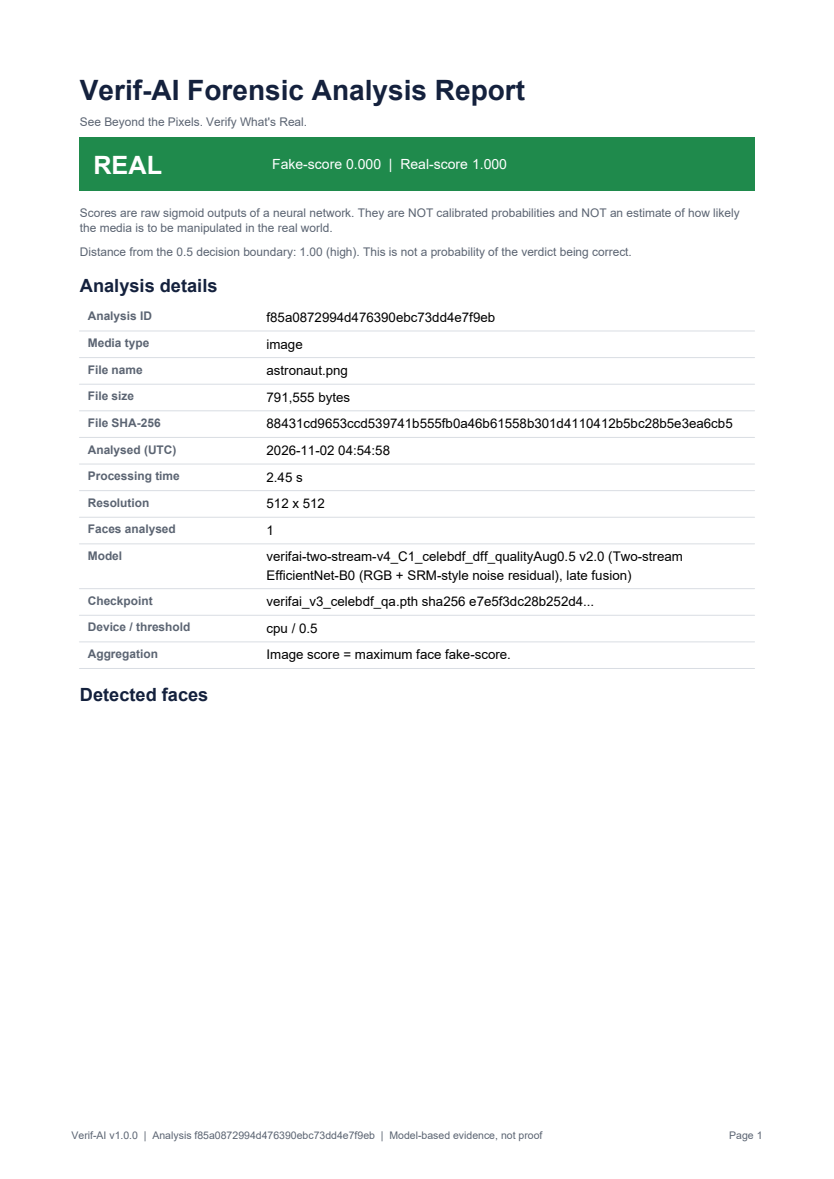
\includegraphics[width=\linewidth,height=1.4137\linewidth]{screenshots/17_pdf_report_p1.png}\caption{Page 1}\end{subfigure}\hfill
\begin{subfigure}[t]{0.47\linewidth}\centering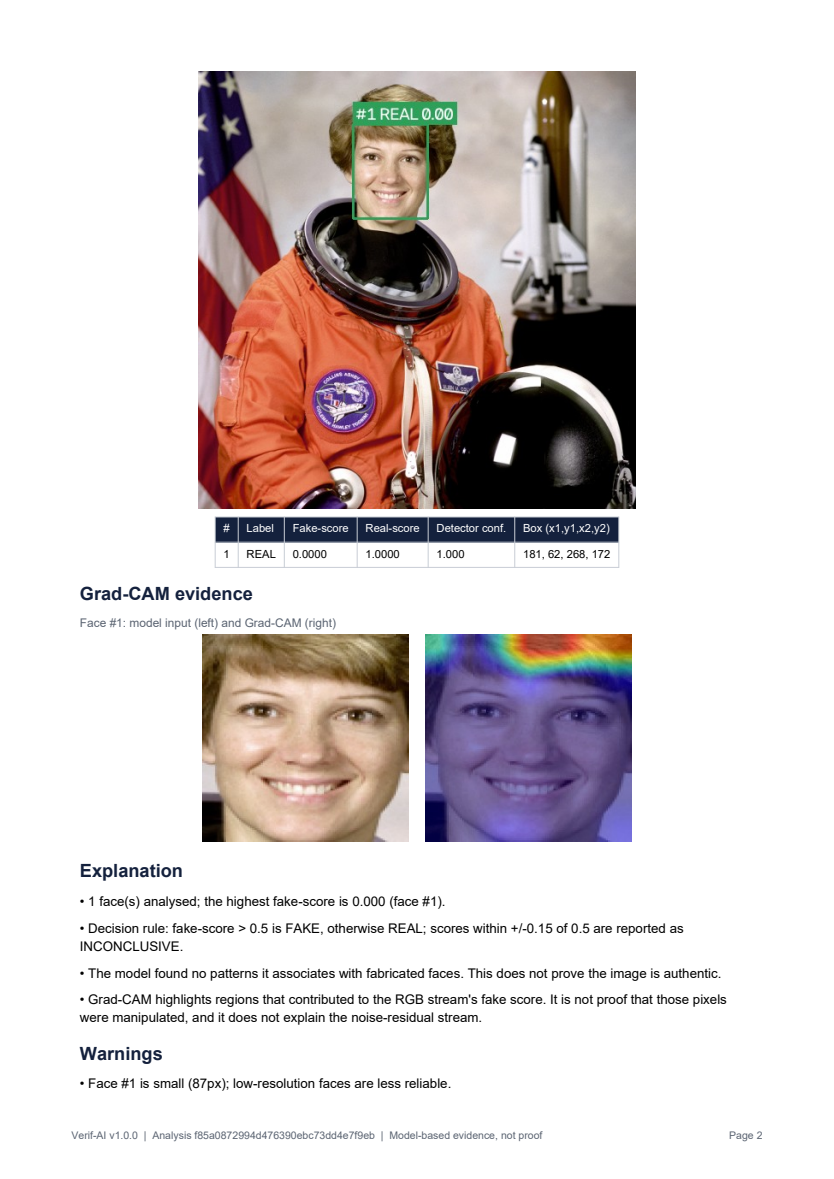
\includegraphics[width=\linewidth,height=1.4137\linewidth]{screenshots/17_pdf_report_p2.png}\caption{Page 2}\end{subfigure}
\caption[Pages 1 and 2 of a PDF forensic report generated by the application for a public test image]{Pages 1 and 2 of a PDF forensic report generated by the application for a public test image. The report records the verdict, the
uncalibrated-score statement, the file and checkpoint hashes and the detected face. (In this version the ``Detected faces'' heading is
separated from its image by a page break, a minor layout flaw.)}
\label{fig:pdf}
\end{figure}

\subsection{Training and Evaluation Implementation}
\textbf{Data preparation.} The DeepFakeFace subset was sampled with one fake counterpart per real image, cropped with the production
detector and split by \emph{identity and pair} so that no person appears in two splits; exact and perceptual duplicates were removed and the
split disjointness was verified by a validation script before training. Celeb-DF videos were split by identity and fakes that cross splits
were dropped. For experiment E3 the splits are file-disjoint and near-duplicates of training crops are removed from validation and test with a
64-bit difference hash (Hamming distance $\le3$).

\textbf{Training.} All models use AdamW \citep{loshchilov2019adamw} with learning rate $10^{-4}$, batch size 32, binary cross-entropy with logits
(positive-class weight set from the training class counts: 1.02 for the DeepFakeFace runs, 0.82 in E4), a learning-rate schedule that reduces on plateau, gradient clipping at 5, at most 12--15 epochs and early stopping with patience 4.
The best epoch is chosen on a \emph{validation} metric only. For the production model it is the validation ROC-AUC; for later experiments with degraded inputs it
is the mean of the clean and degraded validation ROC-AUC. Quality augmentation randomly applies blur, down-up resampling, JPEG compression, noise or low-light degradation.
Training ran in private Kaggle notebooks on a Tesla T4; only checkpoints and metrics were exported from notebooks that used third-party data.

\textbf{Evaluation tooling.} The evaluation script reports accuracy, precision, recall, F1, ROC-AUC, PR-AUC, confusion matrices and error rates
with grouped-bootstrap intervals, per generator and per split, at the fixed threshold, optionally under class-blind degradations; further
tools measure image sharpness bins, stream-level behaviour, an acceptance gate and video-level metrics.

\subsection{Frontend Implementation}
The dashboard is a React/TypeScript single-page application with hash routes, so a refresh or a deep link works on any static host. The
upload card validates the file type and size, detects images versus videos from the extension, shows a preview and calls the image or the video endpoint.
The result page is assembled only from fields of the API response; nothing is mocked or hard-coded.

\textbf{Heat-map viewer for images.} For each detected face the viewer shows the original face crop and the Grad-CAM image side by side, or
one of them alone, or an \emph{overlay} that blends the Grad-CAM image over the crop with an adjustable strength (Figure~\ref{fig:viewer}). Both
images are artifacts produced by the server; the interface does not compute or approximate a heat-map. If several faces are detected a selector
chooses which face is shown, and each face's verdict, score and detector confidence are displayed with it.

\begin{figure}[ht]
\centering
\begin{subfigure}[t]{0.47\linewidth}\centering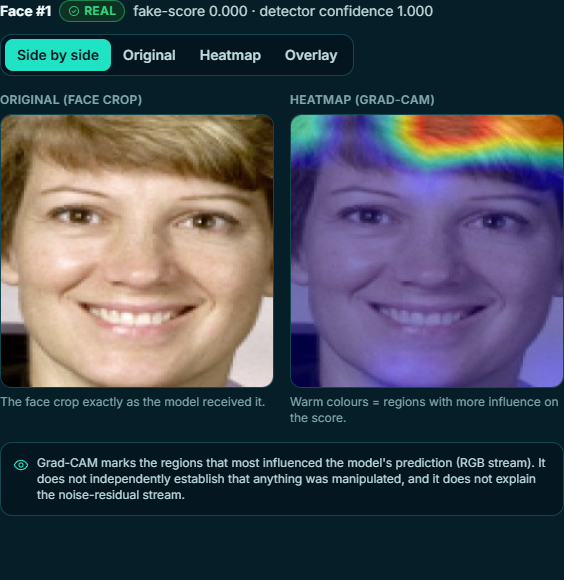
\includegraphics[width=\linewidth,height=1.0284\linewidth]{screenshots/pair_06_side_by_side.png}\caption{Side by side}\end{subfigure}\hfill
\begin{subfigure}[t]{0.47\linewidth}\centering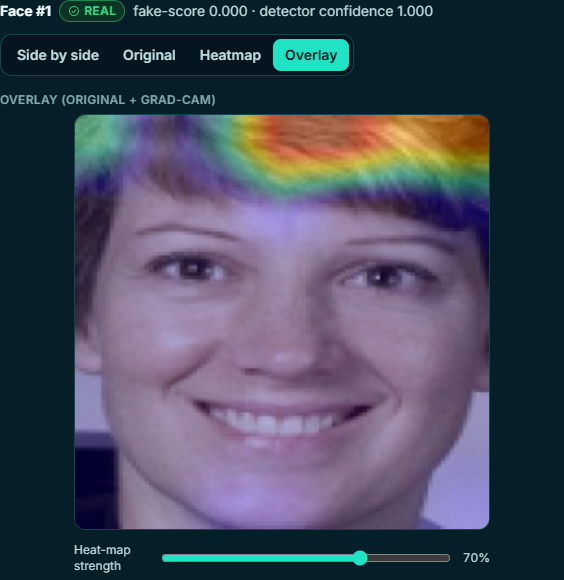
\includegraphics[width=\linewidth,height=1.0284\linewidth]{screenshots/pair_06d_overlay.png}\caption{Overlay (70\% strength)}\end{subfigure}
\caption[Heat-map viewer for an image result (public test image)]{Heat-map viewer for an image result (public test image). The viewer also offers Original-only and Heatmap-only views. The text
under the viewer states that Grad-CAM marks regions that influenced the model and does not establish manipulation.}
\label{fig:viewer}
\end{figure}

\textbf{Frame viewer for videos.} The timeline plots one dot per analysed frame; a dot is selectable. The selected frame's stored
image and heat-map come from the same evidence entry, so they cannot drift apart. Frames without stored evidence show an explicit notice and a
link to the nearest stored frame (Figure~\ref{fig:frames}). Selecting a suspicious time range jumps to the highest-scoring frame in it. The overlay
mode is disabled for video because the server stores the heat-map of the face crop but not its exact position in the frame, and a registered
overlay would be an approximation.

\begin{figure}[ht]
\centering
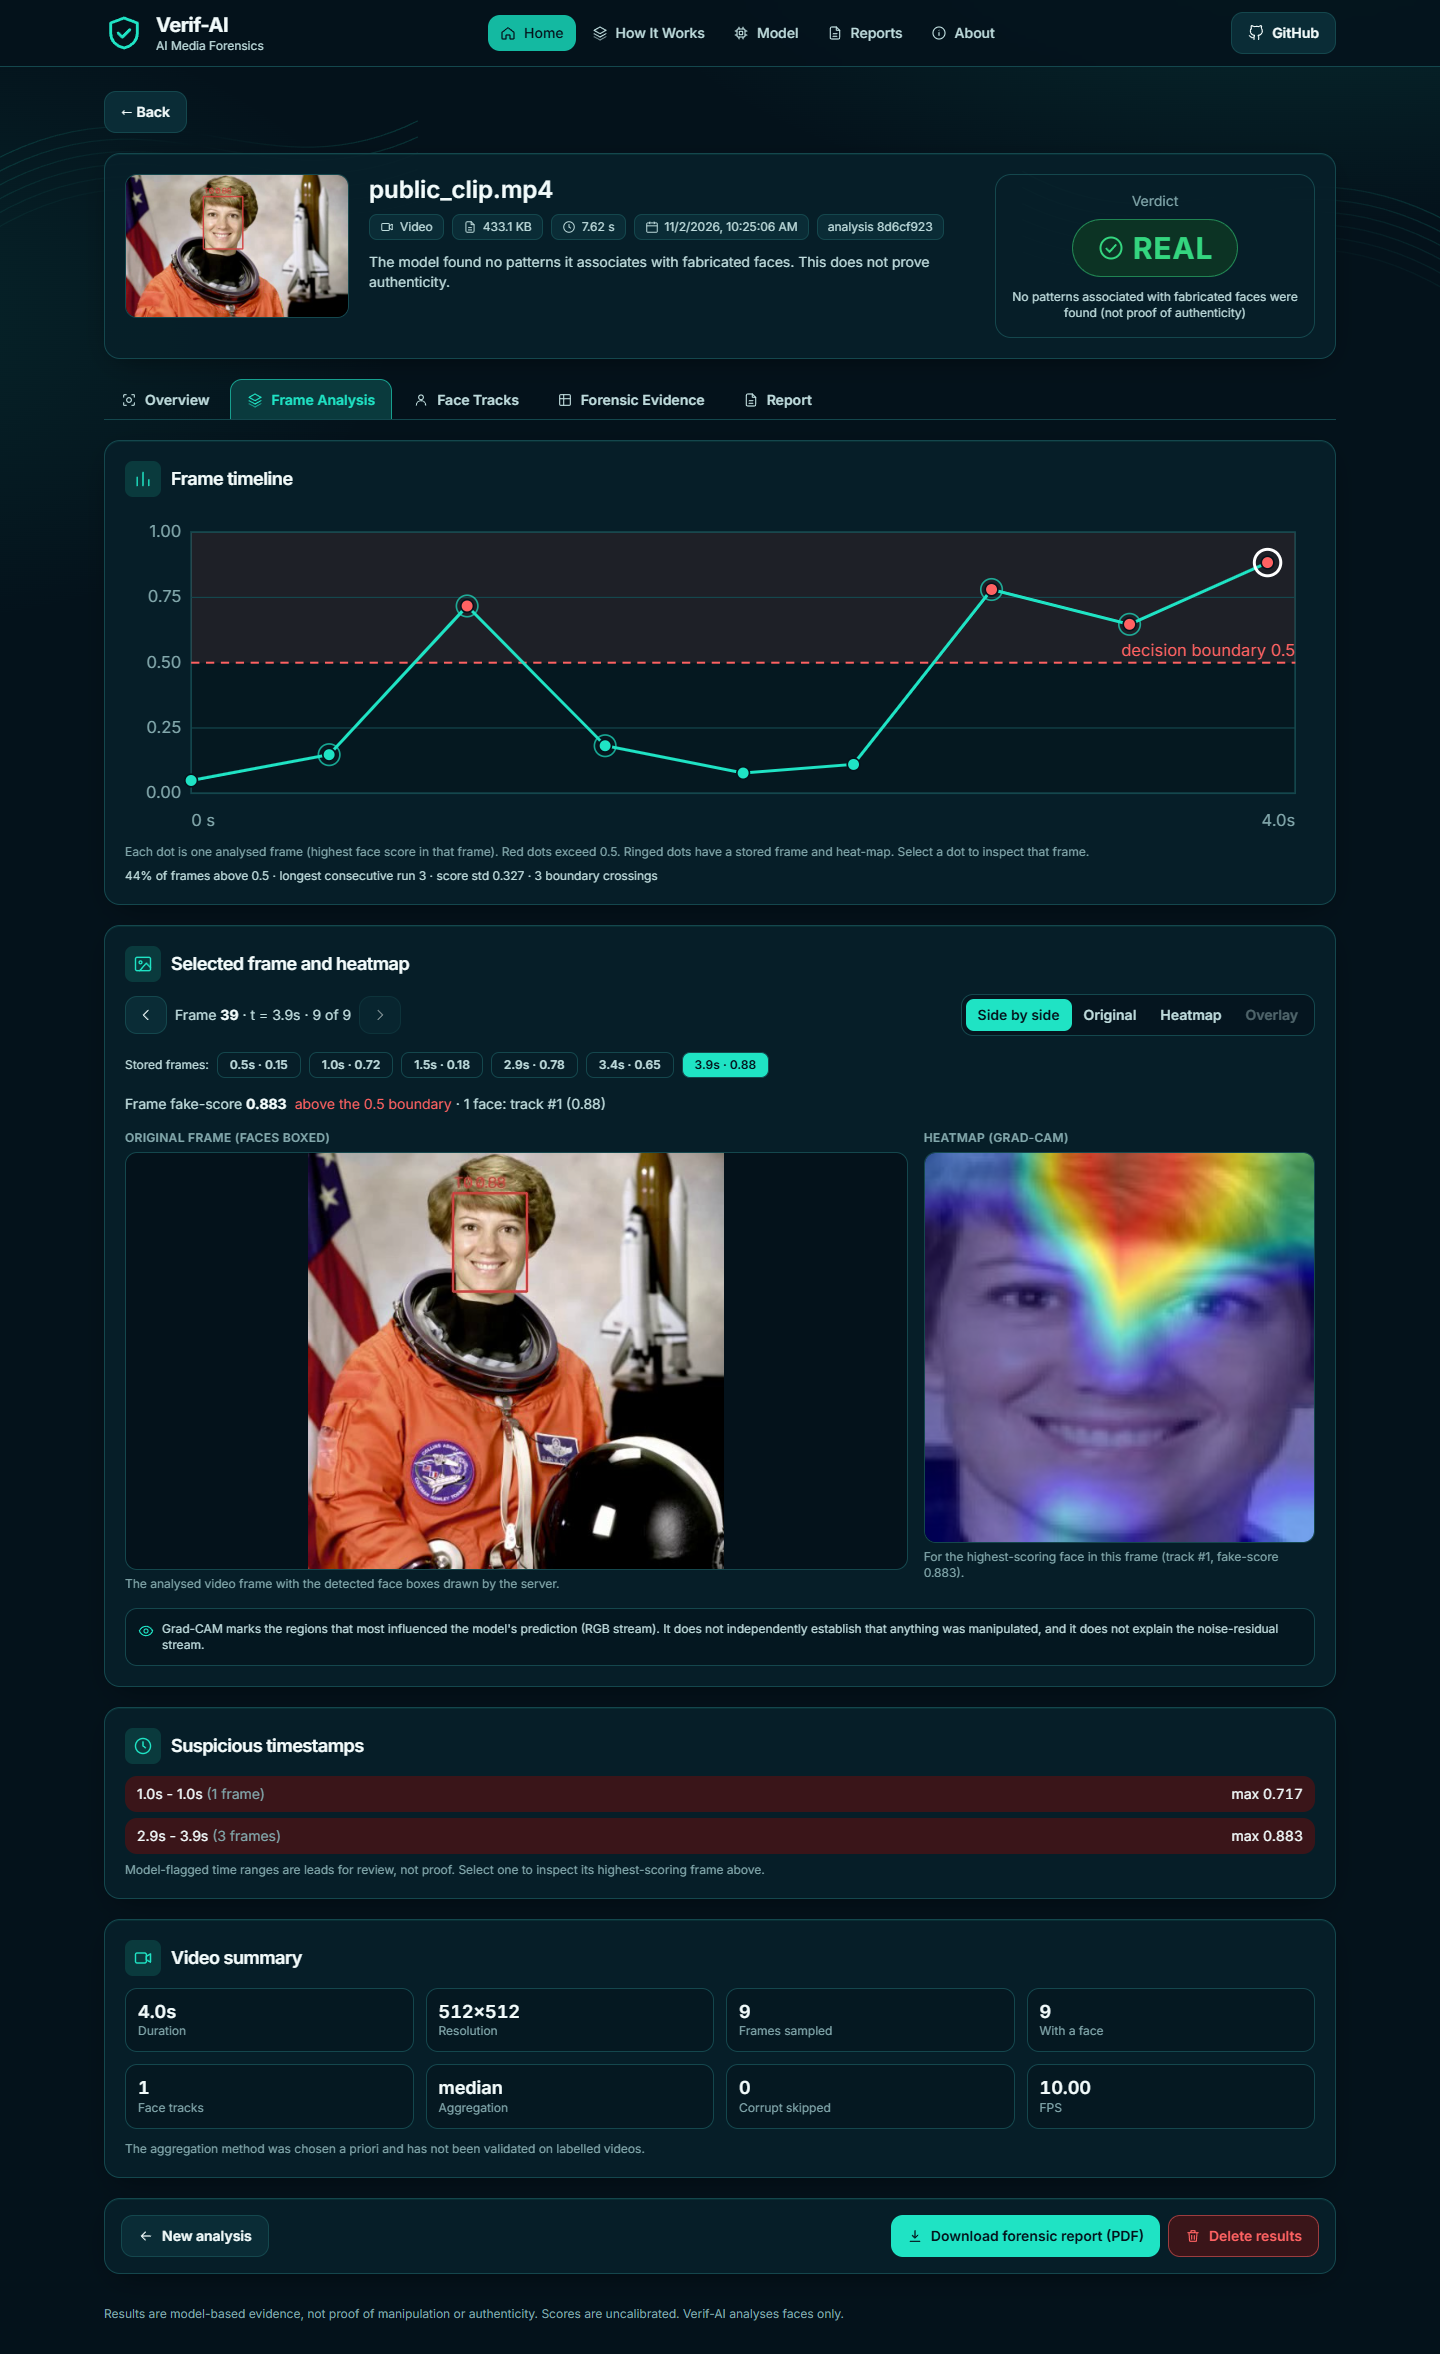
\includegraphics[width=0.96\linewidth,height=0.42\textheight,keepaspectratio]{screenshots/11_video_frame_analysis.png}
\caption[Frame Analysis tab for a video (a synthetic clip made from the public test image): the]{Frame Analysis tab for a video (a synthetic clip made from the public test image): the clickable timeline with the 0.5 decision
boundary, the selected frame with the face boxes and its Grad-CAM, and the stored-frame shortcuts.}
\label{fig:frames}
\end{figure}

\begin{figure}[ht]
\centering
\begin{subfigure}[t]{0.9\linewidth}\centering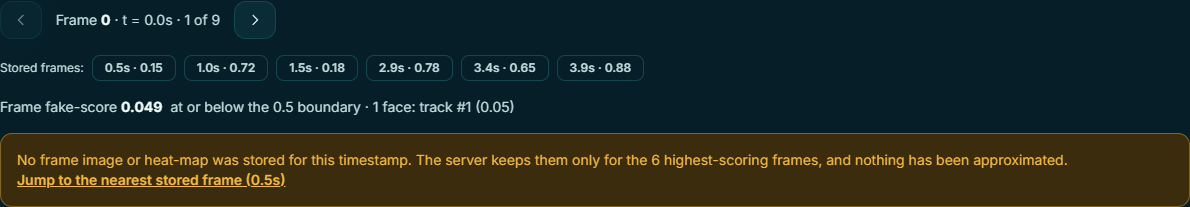
\includegraphics[width=\linewidth,height=0.17395\linewidth]{screenshots/pair_12_not_stored.png}\caption{Frame without stored evidence}\end{subfigure}\\[6pt]
\begin{subfigure}[t]{0.9\linewidth}\centering
\includegraphics[width=\linewidth,height=0.17395\linewidth]{screenshots/pair_13_face_tracks.png}\caption{Face Tracks tab (the card shown on the Face Tracks tab)}\end{subfigure}
\caption[Honest unavailability and face tracks]{Honest unavailability and face tracks. (a) The server keeps frames and heat-maps only for the six highest-scoring frames; other
frames say so. (b) Tracks with frame counts, time span, median score and the share of frames above 0.5.}
\label{fig:notstored}
\end{figure}

\begin{figure}[ht]
\centering
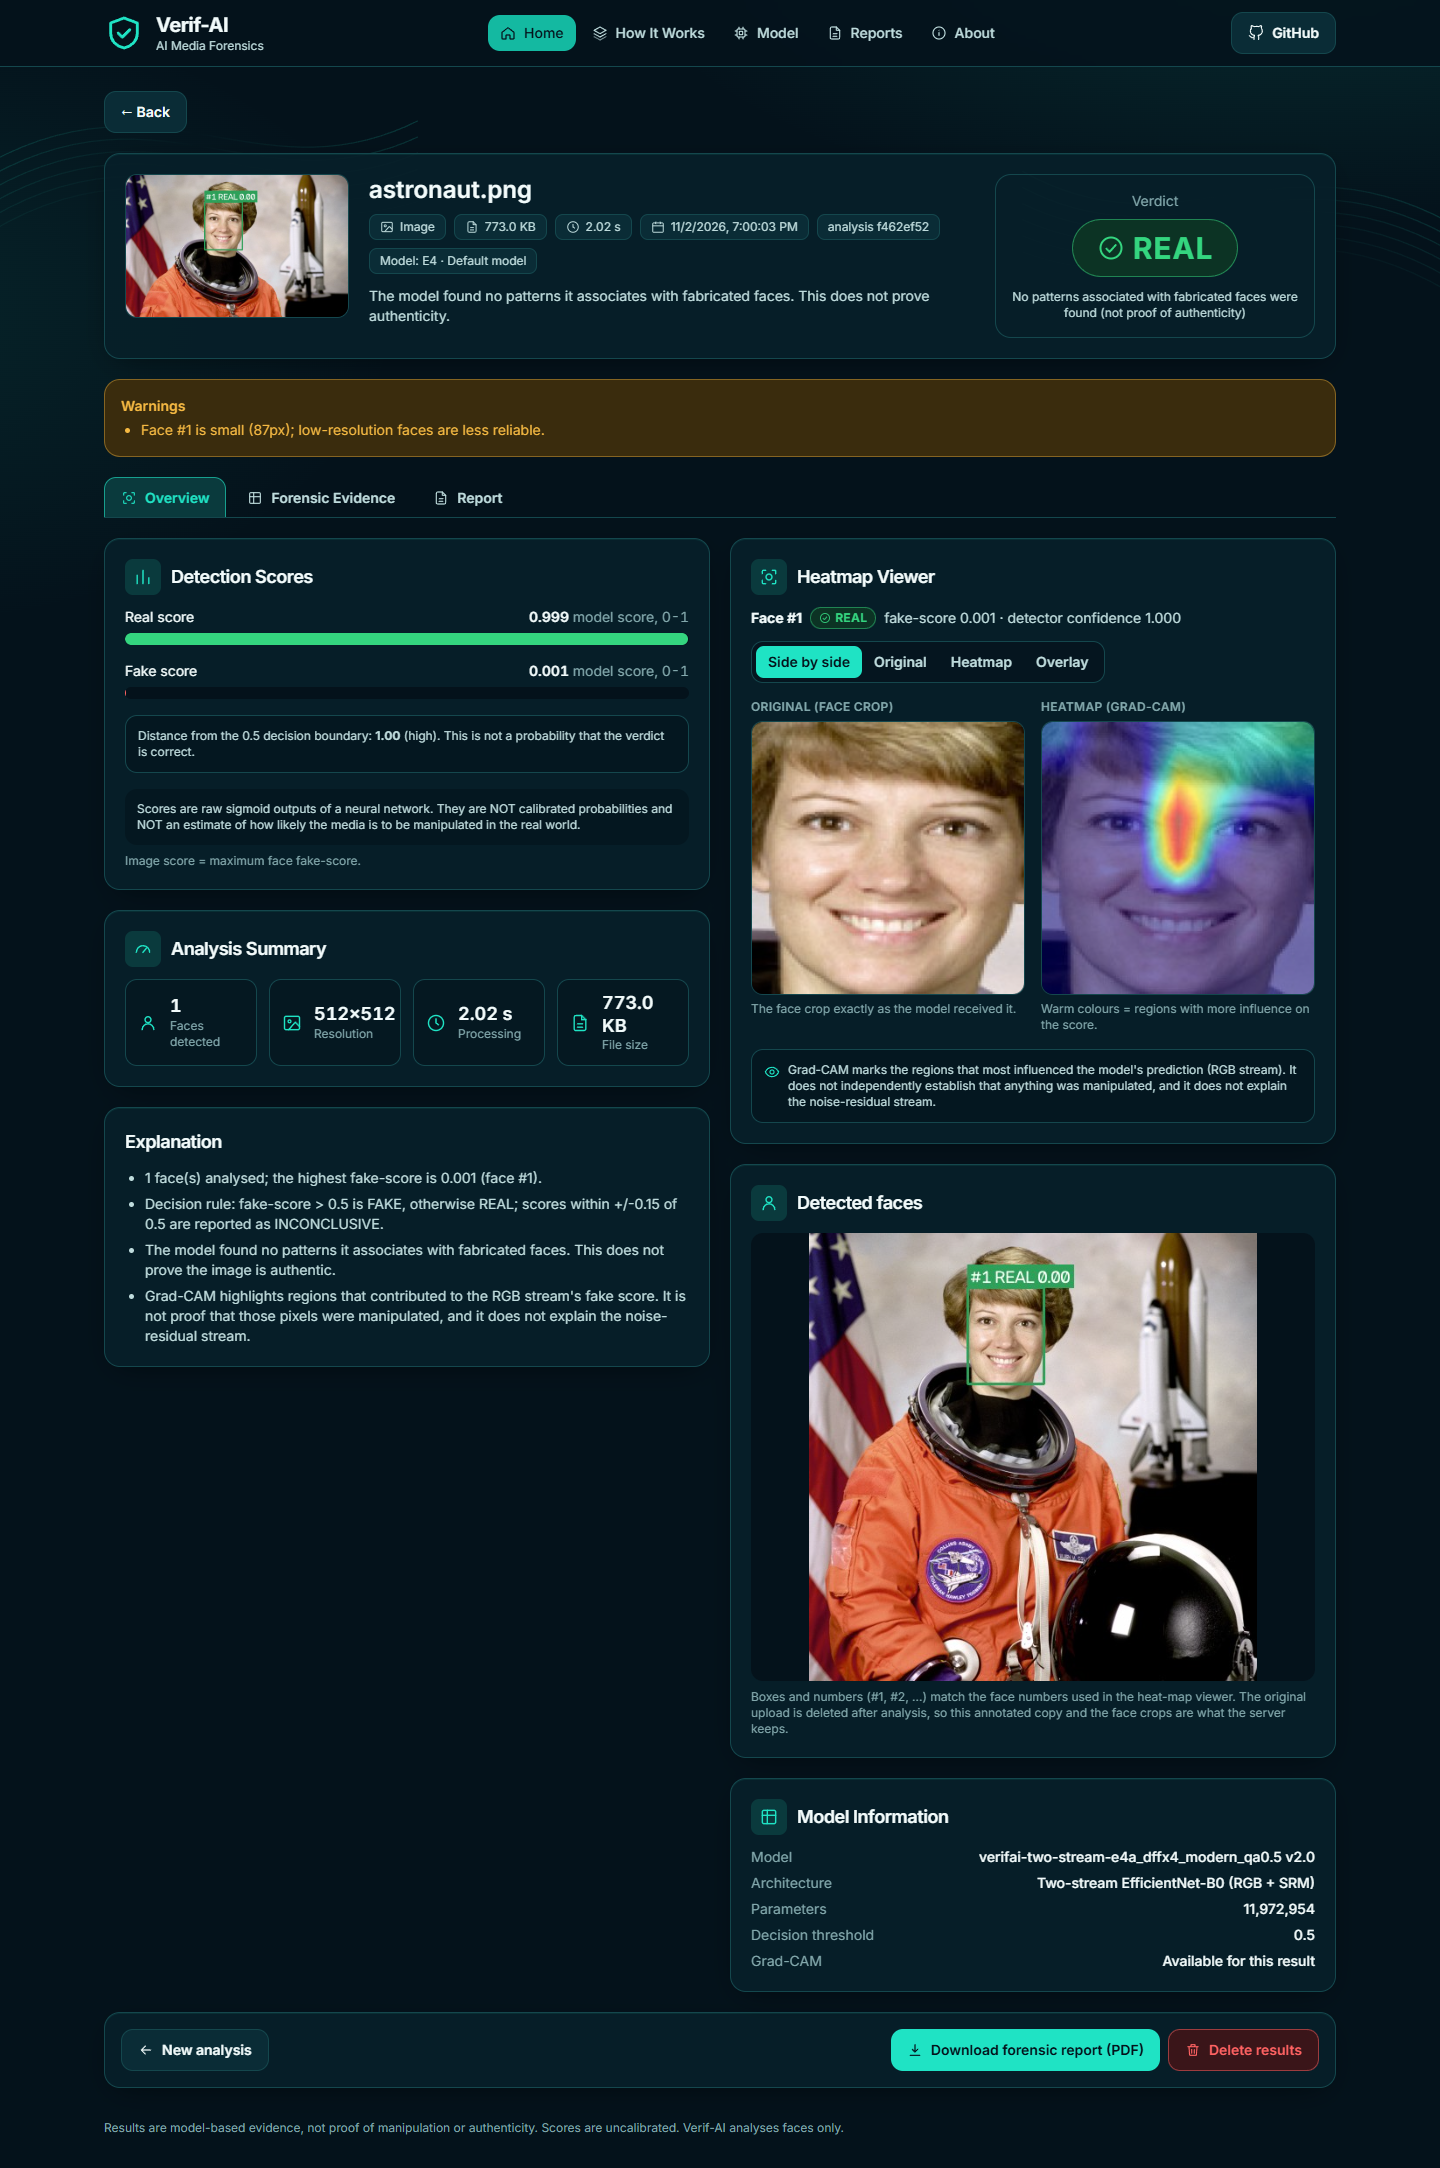
\includegraphics[width=0.96\linewidth,height=0.42\textheight,keepaspectratio]{screenshots/05_image_result_overview.png}
\caption[Overview tab of an image result: verdict, model score labelled as uncalibrated, analysis summary, the heat-map viewer and the detected faces with bounding boxes]{Overview tab of an image result: verdict, model score labelled as uncalibrated, analysis summary, the heat-map viewer and the detected
faces with bounding boxes. The ``Trained On'' text in the model panel (Figure~\ref{fig:ui-home}) is the checkpoint's own metadata, which
understates the data used for this model (Section~\ref{sec:limits}).}
\label{fig:result}
\end{figure}

\textbf{History and deletion.} Because a public API should not list other visitors' analyses, the dashboard stores the identifiers of the
analyses created in that browser and asks the server for each one; deleted or expired identifiers are dropped. Deleting a result removes
the server-side folder and the local entry.

\subsection{Testing and Verification}
Verification was automated wherever possible. The backend suite covers model loading, data validation, scoring and tracking, the image and
video pipelines, the API, the PDF report, training smoke tests and the research tooling; at the time of writing 152 tests passed and 7 were
skipped because they need a test video, a GPU or private media (the skips are environment-gated and were not hidden). The frontend has 63
unit and component tests (including the viewer modes, frame synchronisation and the unavailable states) and 9 Playwright end-to-end tests that
drive a real Chrome browser: unified upload, image and video analysis, heat-map modes, timeline selection, PDF download, deletion, rejected
files, navigation and refresh, console errors and layouts from 1440 to 320 pixels wide. The end-to-end suite was run against the local server, against a separate
frontend origin and against the public deployment.

\subsection{Deployment Implementation}
\label{sec:deploy-impl}
\textbf{Frontend.} The frontend is deployed on Vercel as a static build; \code{vercel.json} fixes the build command and output directory and adds
security headers, and the API address is the build-time variable \code{VITE_API_BASE_URL}. Direct navigation and a refresh were verified on
the public URL.

\textbf{Backend.} The API runs in a Docker container on Render's free tier with CORS limited to the Vercel origin. The memory needed by the
backend was measured on the development laptop (Table~\ref{tab:memory}).

\begin{table}[ht]
\centering
\caption[Backend memory (process working set, MB) measured on the development laptop for different]{Backend memory (process working set, MB) measured on the development laptop for different configurations.}
\label{tab:memory}
\small
\begin{adjustbox}{max width=\linewidth,center}
\begin{tabular}{|p{5.6cm}|c|c|c|}
\hline
\textbf{Configuration} & \textbf{Idle} & \textbf{Image peak} & \textbf{Video peak} \\ \hline
Default (Grad-CAM on, batch 16) & 491 & 776 & over 818 \\ \hline
Grad-CAM on, batch 2, one thread & 488 & 672 & 1473 \\ \hline
Grad-CAM off, batch 2, one thread & 488 & 510 & 576 \\ \hline
\end{tabular}
\end{adjustbox}
\end{table}

A 512\,MB instance cannot run the default configuration: the first analysis on the free tier returned HTTP 502 (the process was killed for lack of memory). The
public instance therefore runs in a restricted ``lite'' mode with Grad-CAM disabled, small batches, a single thread and small upload limits; the
interface reports that heat-maps are unavailable instead of failing. It serves the model checkpoint contained in the repository (v2) because
the newer checkpoint is not stored in Git and the free tier has no persistent disk. Results disappear when the instance restarts and the first
request after an idle period takes about a minute. \textbf{This deployment is a restricted demonstration, not a production system;} full
functionality needs at least 2\,GB of memory and a disk, authentication and rate limiting.

\subsection{Engineering Challenges and Optimisations}
\begin{itemize}
\item \textbf{Identical preprocessing.} Training crops had been stored as JPEG, so inference reproduces the JPEG round-trip; without it the scores
differ from the evaluated ones.
\item \textbf{Leakage control.} Identity-disjoint splits and duplicate removal were implemented before training; later experiments add near-duplicate
removal across training, validation and test (179 validation and 373 test crops were removed in E3).
\item \textbf{Memory.} The memory profile above led to configurable batch sizes, optional Grad-CAM and the lite mode.
\item \textbf{Privacy.} Deleting uploads in all code paths, expiring results and removing the public history list required changes in
both backend and frontend.
\item \textbf{Third-party data.} Notebooks that use third-party images export only checkpoints and metrics; a failed run's output can contain
working files, so logs were read through the API without downloading outputs.
\end{itemize}
